\documentclass[10pt]{article}
\usepackage[margin=0.62in]{geometry}
\usepackage{booktabs,enumitem,fancyhdr,graphicx,tabularx,titlesec}
\usepackage[hidelinks]{hyperref}
\graphicspath{{docs/lessons/assets/}{../assets/}}
\hypersetup{pdftitle={ADK Lesson 052: Copied Infrared Evidence},
 pdfauthor={Kevin Shanahan},
 pdfsubject={Bounded copied pulse evidence, categorical strength, provenance, and deterministic replay},
 pdflang={en-US}}
\pagestyle{fancy}\fancyhf{}
\lhead{\textsc{ADK Lesson 052}}\rhead{Copied Infrared Evidence}
\cfoot{\thepage}\setlength{\headheight}{14pt}
\setlength{\parindent}{0pt}\setlength{\parskip}{3pt}
\setlist{nosep,leftmargin=1.45em}
\titleformat{\section}{\Large\bfseries}{\thesection}{0.5em}{}
\newcommand{\lessonbox}[1]{\begin{center}\fbox{\parbox{0.92\linewidth}{#1}}\end{center}}
\newcommand{\blankline}{\rule{0.78in}{0.4pt}}

\begin{document}
\small
\begin{center}
 {\Huge\bfseries Copied Infrared Evidence}\\[3pt]
 {\Large Preserve what a bounded Lesson 025 frame can actually prove}\\[7pt]
 \fbox{\textbf{E0 COPIED REPLAY --- NO RECEIVER, PIN, OR OPTICAL CLAIM}}
\end{center}
\begin{tabularx}{\linewidth}{@{}>{\bfseries}l X >{\bfseries}l X@{}}
Lesson & 052 --- component & Time & 100--140 minutes\\
Prerequisite & Lesson 025 & Board & compile-only Mega replay\\
Evidence & caller-owned words and result cells & Boundary & no capture hardware\\
\end{tabularx}

\lessonbox{\textbf{Responsibility.} \texttt{CapturedIrEvidence} synchronously
copies one borrowed Lesson 025 pulse frame into fixed caller-owned storage,
classifies it, and publishes attributable evidence. It does not retain the
borrowed view, decode an unknown protocol, operate a receiver, or grant
transmission authority.}

\section{Copy before acknowledging the producer}
A Lesson 025 view is borrowed. While it is valid, copy every significant
duration and mark bit into the configured destination. Reject a frame that is
empty, too long, truncated, overflowed, malformed, or not representable in
the fixed storage. Only after the copy and classification are complete may
the caller acknowledge the producer.

\begin{center}
% ADK visual: pencil
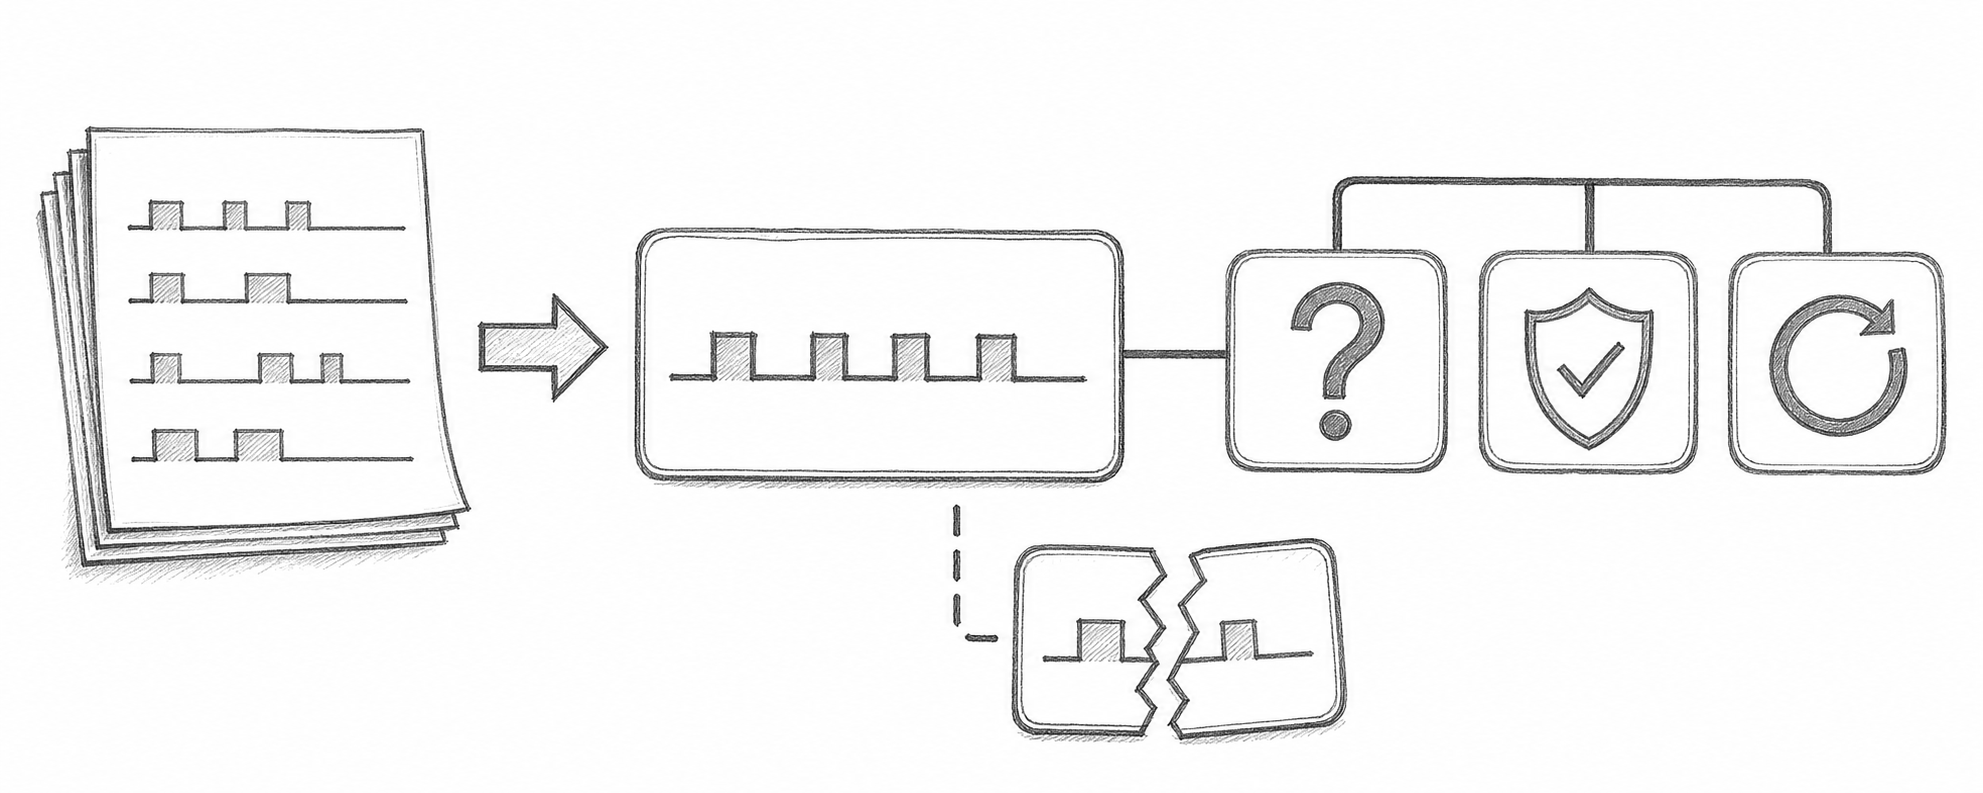
\includegraphics[width=0.98\linewidth,height=0.30\textheight,
 keepaspectratio]{052-copied-evidence-pencil.png}

\small\textit{Alternative text: graphite pulse sheets enter one bounded
copied record, which branches to question-mark, shield-check, and repeat
cards. A broken pulse card below is separated from the accepted path.}
\end{center}

The drawing is a conceptual memory-flow mnemonic. It contains no receiver,
wiring, carrier, pin assignment, or formal schematic.

\section{Use categorical evidence, never invented confidence}
\begin{tabularx}{\linewidth}{@{}l X X@{}}
\toprule
Strength & What the copied record supports & What it cannot support\\
\midrule
\texttt{None} & no usable qualified observation & protocol or command claim\\
\texttt{ShapeRecognized} & bounded structure resembles the known shape &
integrity or transmit authority\\
\texttt{IntegrityVerified} & the configured decoder verified the known
record's integrity & physical origin, user intent, or safe actuation\\
\bottomrule
\end{tabularx}

Repeat is a distinct disposition, not a stronger command. Unknown, malformed,
overflowed, truncated, stale, and repeat records remain inspectable but never
inherit the authority of an earlier valid record.

\section{Bind evidence to its source and generation}
Each accepted snapshot retains source kind and ID, configuration revision,
qualification epoch, occurrence and observation times, source sequence,
decoder disposition, categorical strength, significant word count, and a
digest of the complete copied payload. A same-sequence byte-identical replay
is idempotent. Changed content at the same sequence is malformed.

Forward sequence order and elapsed time use unsigned modular half-range
comparison. Exact-half-range ambiguity rejects; rollover alone is not a
fault. Stale, future, regressing, source-changing, or configuration-changing
input does not partly replace the last accepted evidence.

\begin{tabularx}{\linewidth}{@{}l X@{}}
\toprule
Case & Predict before replay\\
\midrule
known valid frame & copied view, \texttt{IntegrityVerified}, new generation\\
recognized shape with failed integrity & inspectable, no valid command\\
repeat record & repeat disposition, no inherited authorization\\
unknown bounded frame & copied for diagnosis, never emission input\\
overflow or truncation & atomic rejection; no partial record\\
same sequence, changed pulse & malformed; accepted history preserved\\
\bottomrule
\end{tabularx}

\newpage
\section{Run the deterministic workbook}
Use the canonical compile-only Lesson 052 sketch and executable host tests.
Predict each named result cell before inspecting it.

\begin{enumerate}
 \item Initialize with fixed caller storage and a nonzero instance epoch.
       Predict inactive lifecycle, zero copied words, and no evidence.
 \item Admit one known valid synthetic frame. Record disposition, strength,
       source sequence, evidence generation, and digest.
 \item Replay it byte-for-byte at the same sequence, then change one duration.
       Distinguish idempotence from malformed mutation.
 \item Supply shape-recognized, repeat, unknown, malformed, truncated, and
       overflowed frames. Verify that each remains categorically distinct.
 \item Exercise exact freshness boundaries, timestamp rollover, regression,
       future observation, and half-range ambiguity.
 \item Change source ID, configuration revision, and qualification epoch.
       Verify provenance checks before any snapshot mutation.
 \item Reset and restart. Confirm that old evidence and old generations do
       not silently become current.
\end{enumerate}

\begin{tabularx}{\linewidth}{@{}X X X X X@{}}
\toprule
frame & disposition & strength & words & generation\\
\midrule
\rule{0pt}{16pt}\blankline & \blankline & \blankline & \blankline & \blankline\\[8pt]
\blankline & \blankline & \blankline & \blankline & \blankline\\[8pt]
\blankline & \blankline & \blankline & \blankline & \blankline\\
\bottomrule
\end{tabularx}

\section{Separate acquisition evidence from safe-state evidence}
\textbf{Acquisition prediction.} Valid extents, non-overlapping caller
storage, supported source constraints, and a nonzero epoch allow E0
initialization.

\textbf{Acquisition observation.} Host tests inspect lifecycle status,
copied-word count, provenance, digest, disposition, strength, and generation
in memory.

\textbf{Acquisition interpretation.} Success proves bounded copying and
classification only. It does not prove a receiver, interrupt, pin, carrier,
optical signal, remote identity, or physical Mega execution.

\textbf{Safe-state prediction and observation.} Construction, failed
initialization, reset, fault, and shutdown publish no current valid evidence
and cannot produce emission intent. This is software state, not proof that a
future electrical endpoint is unpowered.

\section{Read the conservative resource evidence}
The final canonical Mega 2560 sketch measures 5,530 bytes of flash and
1,096 bytes of static SRAM with Arduino AVR core 1.8.8 and avr-gcc 7.3.0.
\texttt{sizeof(CapturedIrEvidence)} is 48 bytes. Conservative compiler stack
evidence estimates about 197 bytes on the measured deepest analyzed path.

These numbers are compiler evidence for this exact source, toolchain,
optimization, and fixture. They are not runtime high-water measurements,
proof of stack safety under every interrupt schedule, or a powered-hardware
claim. Re-measure whenever the sketch, library, core, compiler, flags, or
composition changes.

\section{Keep E1 explicitly open}
An E1 adapter needs an exact receiver specimen, primary evidence, voltage and
timing limits, qualified pin and interrupt ownership, a formal authoritative
schematic, acquisition rollback, non-Serial observation, and recorded bench
acceptance. None is supplied here. Phone-camera observations are not receiver
qualification.

\section{Evidence and next step}
Compare the compile-only Mega result cells with the deterministic component
tests and the accessible HTML lesson. Record:

\begin{itemize}
 \item acquisition status: \blankline\quad evidence generation: \blankline
 \item copied count: \blankline\quad disposition: \blankline
 \item strength: \blankline\quad safe-state result: \blankline
\end{itemize}

Lesson 053 accepts only a fixed locally authored symbolic catalog. No
\texttt{CapturedIrView}, copied pulse, raw duration, unknown command, or
repeat record can enter that catalog.

\end{document}
